\documentclass[twoside]{book}

% Packages required by doxygen
\usepackage{calc}
\usepackage{doxygen}
\usepackage{graphicx}
\usepackage[utf8]{inputenc}
\usepackage{makeidx}
\usepackage{multicol}
\usepackage{multirow}
\usepackage{textcomp}
\usepackage[table]{xcolor}

% Font selection
\usepackage[T1]{fontenc}
\usepackage{mathptmx}
\usepackage[scaled=.90]{helvet}
\usepackage{courier}
\usepackage{amssymb}
\usepackage{sectsty}
\renewcommand{\familydefault}{\sfdefault}
\allsectionsfont{%
  \fontseries{bc}\selectfont%
  \color{darkgray}%
}
\renewcommand{\DoxyLabelFont}{%
  \fontseries{bc}\selectfont%
  \color{darkgray}%
}

% Page & text layout
\usepackage{geometry}
\geometry{%
  a4paper,%
  top=2.5cm,%
  bottom=2.5cm,%
  left=2.5cm,%
  right=2.5cm%
}
\tolerance=750
\hfuzz=15pt
\hbadness=750
\setlength{\emergencystretch}{15pt}
\setlength{\parindent}{0cm}
\setlength{\parskip}{0.2cm}
\makeatletter
\renewcommand{\paragraph}{%
  \@startsection{paragraph}{4}{0ex}{-1.0ex}{1.0ex}{%
    \normalfont\normalsize\bfseries\SS@parafont%
  }%
}
\renewcommand{\subparagraph}{%
  \@startsection{subparagraph}{5}{0ex}{-1.0ex}{1.0ex}{%
    \normalfont\normalsize\bfseries\SS@subparafont%
  }%
}
\makeatother

% Headers & footers
\usepackage{fancyhdr}
\pagestyle{fancyplain}
\fancyhead[LE]{\fancyplain{}{\bfseries\thepage}}
\fancyhead[CE]{\fancyplain{}{}}
\fancyhead[RE]{\fancyplain{}{\bfseries\leftmark}}
\fancyhead[LO]{\fancyplain{}{\bfseries\rightmark}}
\fancyhead[CO]{\fancyplain{}{}}
\fancyhead[RO]{\fancyplain{}{\bfseries\thepage}}
\fancyfoot[LE]{\fancyplain{}{}}
\fancyfoot[CE]{\fancyplain{}{}}
\fancyfoot[RE]{\fancyplain{}{\bfseries\scriptsize 2016年01月22日(金) 22時34分29秒作成 -\/ E\-V3\-Control\-Client / 構成\-:  Doxygen }}
\fancyfoot[LO]{\fancyplain{}{\bfseries\scriptsize 2016年01月22日(金) 22時34分29秒作成 -\/ E\-V3\-Control\-Client / 構成\-:  Doxygen }}
\fancyfoot[CO]{\fancyplain{}{}}
\fancyfoot[RO]{\fancyplain{}{}}
\renewcommand{\footrulewidth}{0.4pt}
\renewcommand{\chaptermark}[1]{%
  \markboth{#1}{}%
}
\renewcommand{\sectionmark}[1]{%
  \markright{\thesection\ #1}%
}

% Indices & bibliography
\usepackage{natbib}
\usepackage[titles]{tocloft}
\setcounter{tocdepth}{3}
\setcounter{secnumdepth}{5}
\makeindex

% Custom commands
\newcommand{\clearemptydoublepage}{%
  \newpage{\pagestyle{empty}\cleardoublepage}%
}


%===== C O N T E N T S =====

\begin{document}

% Titlepage & ToC
\pagenumbering{roman}
\begin{titlepage}
\vspace*{7cm}
\begin{center}%
{\Large E\-V3\-Control\-Client }\\
\vspace*{1cm}
{\large 構築\-: Doxygen 1.8.6}\\
\vspace*{0.5cm}
{\small 2016年01月22日(金) 22時34分29秒}\\
\end{center}
\end{titlepage}
\clearemptydoublepage
\tableofcontents
\clearemptydoublepage
\pagenumbering{arabic}

%--- Begin generated contents ---
\chapter{階層索引}
\section{クラス階層}
クラス階層一覧です。大雑把に文字符号順で並べられています。\begin{DoxyCompactList}
\item \contentsline{section}{E\-V3\-Control\-Client}{\pageref{class_e_v3_control_client}}{}
\item \contentsline{section}{Run\-Control\-E\-V3}{\pageref{class_run_control_e_v3}}{}
\item \contentsline{section}{Socket\-Client}{\pageref{class_socket_client}}{}
\item Timer\-Task\begin{DoxyCompactList}
\item \contentsline{section}{Run\-Client}{\pageref{class_run_client}}{}
\end{DoxyCompactList}
\end{DoxyCompactList}

\chapter{クラス索引}
\section{クラス一覧}
クラス・構造体・共用体・インターフェースの一覧です。\begin{DoxyCompactList}
\item\contentsline{section}{{\bf E\-V3\-Control\-Client} \\*クライアント側のメインの処理クラス }{\pageref{class_e_v3_control_client}}{}
\item\contentsline{section}{{\bf Run\-Client} \\*クライアント側で連続で行う処理を記述したクラス }{\pageref{class_run_client}}{}
\item\contentsline{section}{{\bf Run\-Control\-E\-V3} \\*E\-V3の走行制御クラス }{\pageref{class_run_control_e_v3}}{}
\item\contentsline{section}{{\bf Socket\-Client} \\*ソケット通信のクライアント側のクラス }{\pageref{class_socket_client}}{}
\end{DoxyCompactList}

\chapter{ファイル索引}
\section{ファイル一覧}
ファイル一覧です。\begin{DoxyCompactList}
\item\contentsline{section}{{\bf E\-V3\-Control\-Client.\-java} \\*E\-V3を制御するクライアント(\-E\-V3)側のメインクラス. }{\pageref{_e_v3_control_client_8java}}{}
\item\contentsline{section}{{\bf Run\-Client.\-java} \\*クライアント(\-E\-V3)側の時間をスケジューリングするクラス. }{\pageref{_run_client_8java}}{}
\item\contentsline{section}{{\bf Run\-Control\-E\-V3.\-java} \\*E\-V3の走行を制御するクラス }{\pageref{_run_control_e_v3_8java}}{}
\item\contentsline{section}{{\bf Socket\-Client.\-java} \\*クライアントクラス.\-E\-V3から送信する\-P\-C側のサーバーへ通信する }{\pageref{_socket_client_8java}}{}
\end{DoxyCompactList}

\chapter{クラス詳解}
\section{E\-V3\-Control\-Client クラス}
\label{class_e_v3_control_client}\index{E\-V3\-Control\-Client@{E\-V3\-Control\-Client}}


クライアント側のメインの処理クラス  


\subsection*{静的公開メンバ関数}
\begin{DoxyCompactItemize}
\item 
static void {\bf main} (String[$\,$] args)
\begin{DoxyCompactList}\small\item\em メインメソッド \end{DoxyCompactList}\end{DoxyCompactItemize}


\subsection{詳解}
クライアント側のメインの処理クラス 

 E\-V3\-Control\-Client.\-java の 15 行目に定義があります。



\subsection{メソッド詳解}
\index{E\-V3\-Control\-Client@{E\-V3\-Control\-Client}!main@{main}}
\index{main@{main}!EV3ControlClient@{E\-V3\-Control\-Client}}
\subsubsection[{main}]{\setlength{\rightskip}{0pt plus 5cm}static void E\-V3\-Control\-Client.\-main (
\begin{DoxyParamCaption}
\item[{String[$\,$]}]{args}
\end{DoxyParamCaption}
)\hspace{0.3cm}{\ttfamily [static]}}\label{class_e_v3_control_client_abc614e9ac31834c5d74fe01affb19383}


メインメソッド 



 E\-V3\-Control\-Client.\-java の 19 行目に定義があります。



このクラス詳解は次のファイルから抽出されました\-:\begin{DoxyCompactItemize}
\item 
{\bf E\-V3\-Control\-Client.\-java}\end{DoxyCompactItemize}

\section{Run\-Client クラス}
\label{class_run_client}\index{Run\-Client@{Run\-Client}}


クライアント側で連続で行う処理を記述したクラス  




Run\-Client の継承関係図
\nopagebreak
\begin{figure}[H]
\begin{center}
\leavevmode
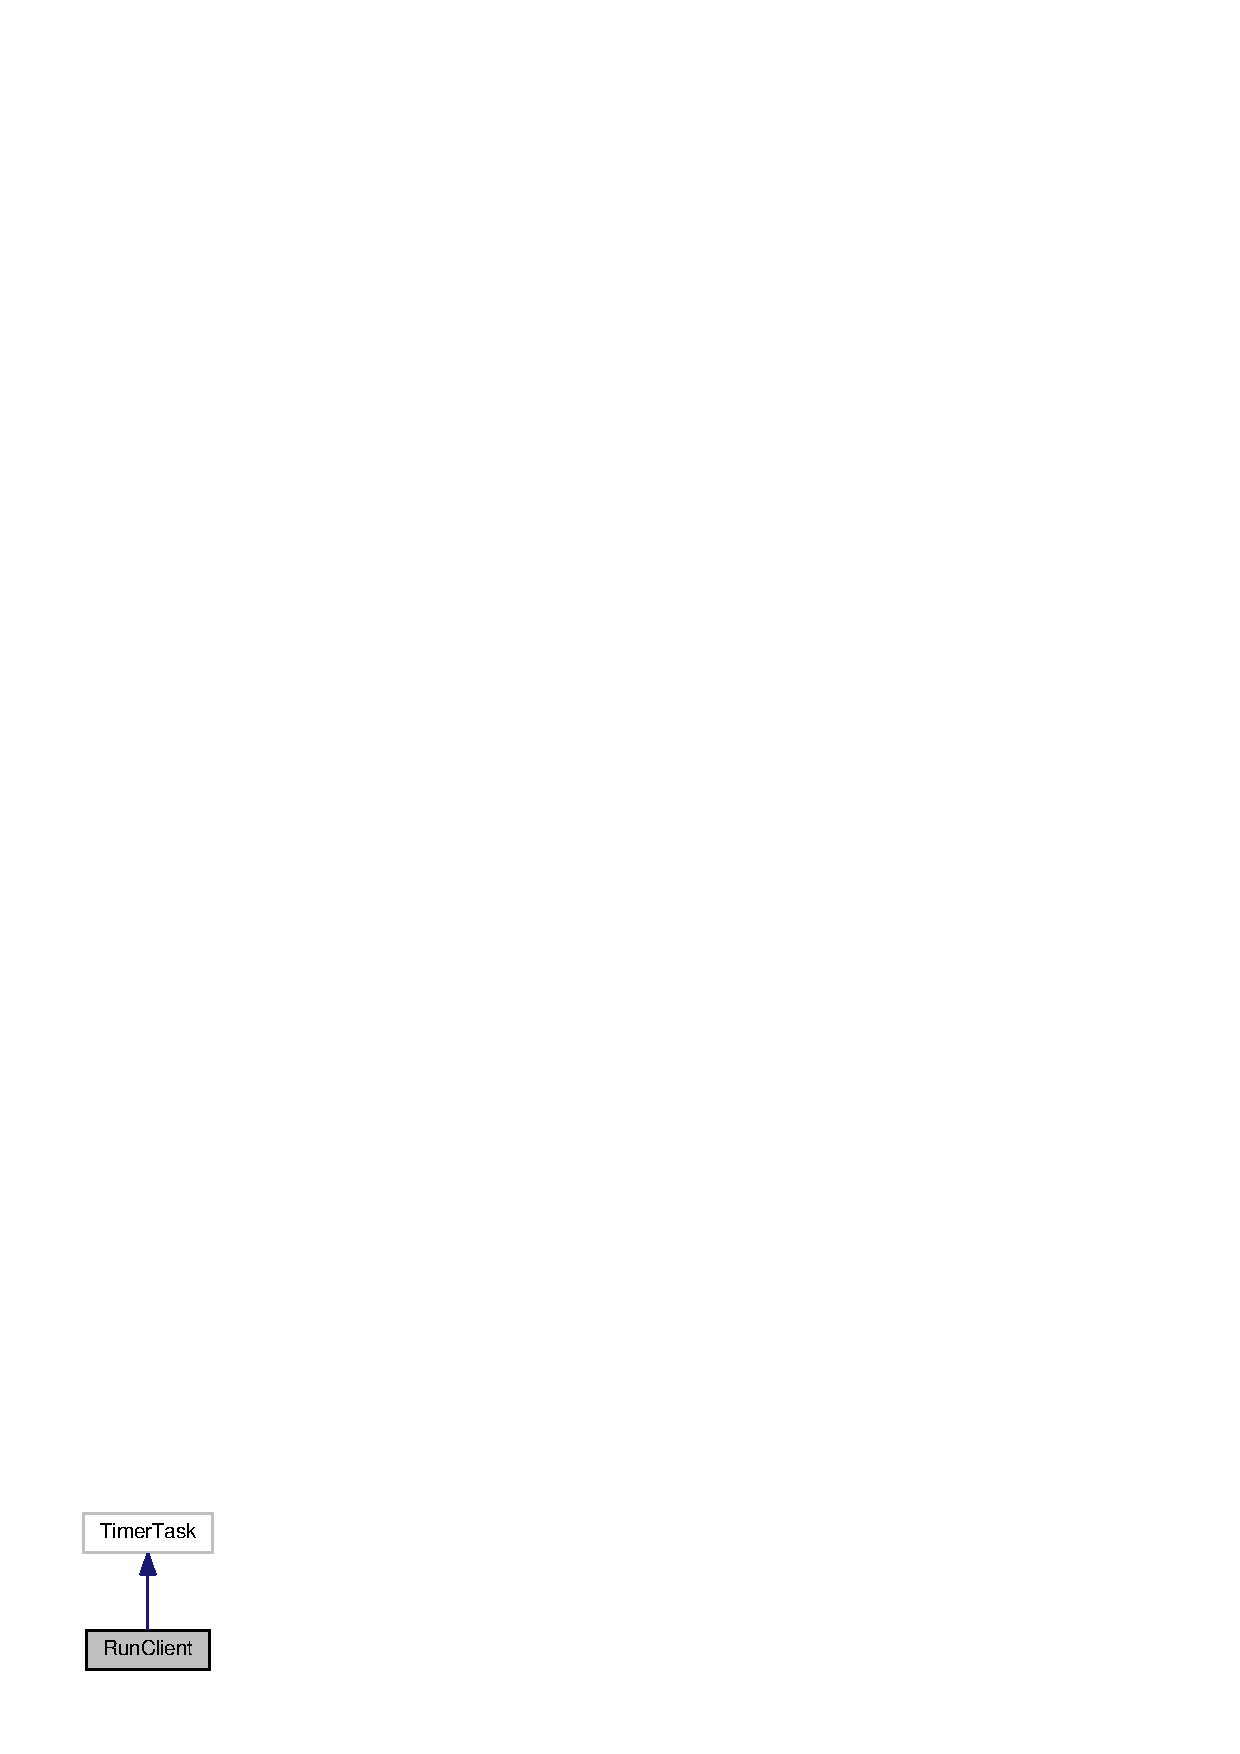
\includegraphics[width=106pt]{class_run_client__inherit__graph}
\end{center}
\end{figure}


Run\-Client 連携図
\nopagebreak
\begin{figure}[H]
\begin{center}
\leavevmode
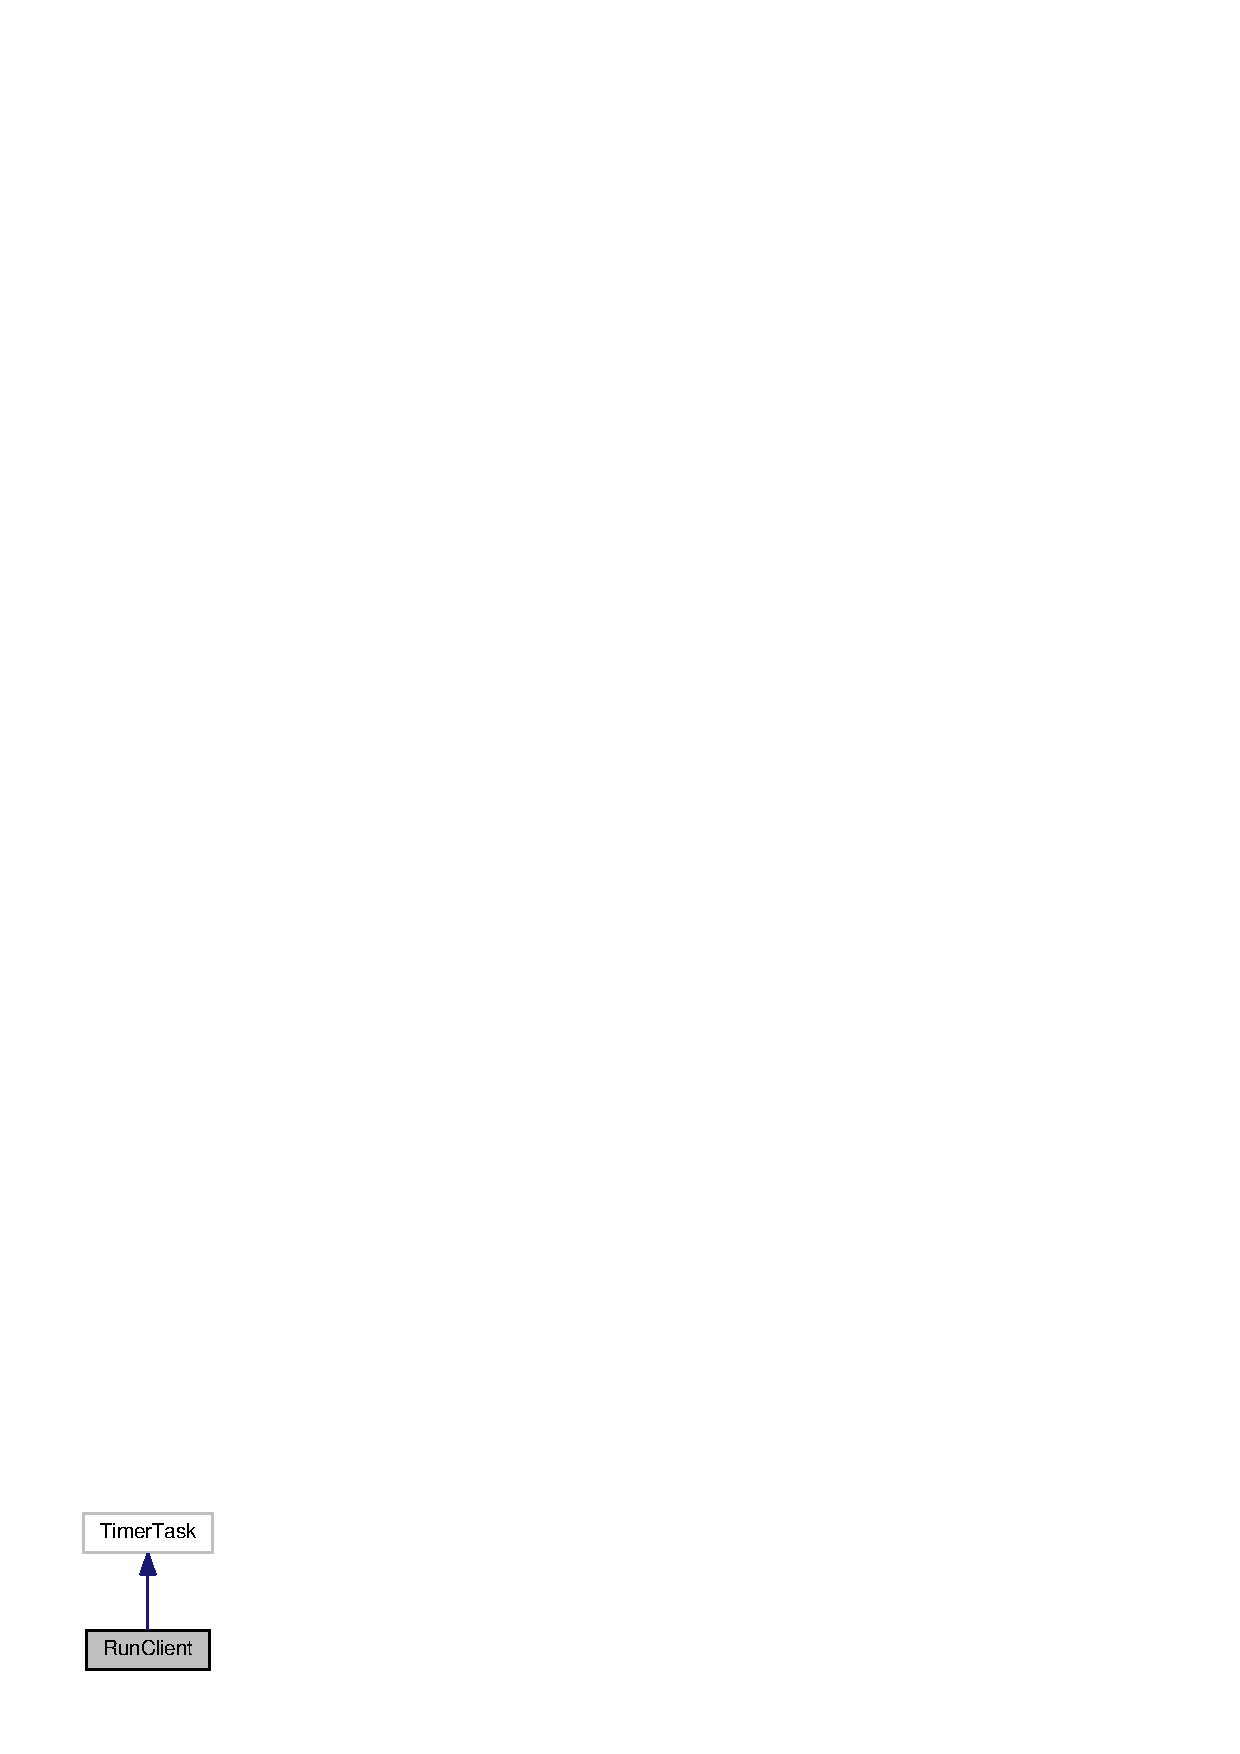
\includegraphics[width=106pt]{class_run_client__coll__graph}
\end{center}
\end{figure}
\subsection*{公開メンバ関数}
\begin{DoxyCompactItemize}
\item 
void {\bf run} ()
\begin{DoxyCompactList}\small\item\em 処理の流れをここに書く \end{DoxyCompactList}\end{DoxyCompactItemize}


\subsection{詳解}
クライアント側で連続で行う処理を記述したクラス 

 Run\-Client.\-java の 19 行目に定義があります。



\subsection{メソッド詳解}
\index{Run\-Client@{Run\-Client}!run@{run}}
\index{run@{run}!RunClient@{Run\-Client}}
\subsubsection[{run}]{\setlength{\rightskip}{0pt plus 5cm}void Run\-Client.\-run (
\begin{DoxyParamCaption}
{}
\end{DoxyParamCaption}
)}\label{class_run_client_a409dd9f6c94f024db9969b2948a7380b}


処理の流れをここに書く 



 Run\-Client.\-java の 34 行目に定義があります。



このクラス詳解は次のファイルから抽出されました\-:\begin{DoxyCompactItemize}
\item 
{\bf Run\-Client.\-java}\end{DoxyCompactItemize}

\section{Run\-Control\-E\-V3 クラス}
\label{class_run_control_e_v3}\index{Run\-Control\-E\-V3@{Run\-Control\-E\-V3}}


E\-V3の走行制御クラス  


\subsection*{公開メンバ関数}
\begin{DoxyCompactItemize}
\item 
void {\bf Calculate\-Input\-Value} (double velocity, double yaw)
\begin{DoxyCompactList}\small\item\em 左右モーターの入力を計算するメソッド(要修正) \end{DoxyCompactList}\item 
void {\bf Control\-E\-V3} (String args[$\,$])
\begin{DoxyCompactList}\small\item\em 実際に入力を与え\-E\-V3を走行させるメソッド \end{DoxyCompactList}\end{DoxyCompactItemize}
\subsection*{静的公開変数類}
\begin{DoxyCompactItemize}
\item 
static int {\bf ul}
\begin{DoxyCompactList}\small\item\em 現在のモーター\-A(左)の角速度 \end{DoxyCompactList}\item 
static int {\bf ur}
\begin{DoxyCompactList}\small\item\em 現在のモーター\-B(右)の角速度 \end{DoxyCompactList}\item 
static int {\bf ul\-\_\-real}
\begin{DoxyCompactList}\small\item\em モーター\-A(左)の実際の角速度 \end{DoxyCompactList}\item 
static int {\bf ur\-\_\-real}
\begin{DoxyCompactList}\small\item\em モーター\-B(右)の実際の角速度 \end{DoxyCompactList}\item 
static boolean {\bf flag\-\_\-once}
\begin{DoxyCompactList}\small\item\em 1回目の処理をチェックするためのフラグ \end{DoxyCompactList}\end{DoxyCompactItemize}


\subsection{詳解}
E\-V3の走行制御クラス 

Aが左のモーターl,\-Bが右のモーターr 

 Run\-Control\-E\-V3.\-java の 20 行目に定義があります。



\subsection{メソッド詳解}
\index{Run\-Control\-E\-V3@{Run\-Control\-E\-V3}!Calculate\-Input\-Value@{Calculate\-Input\-Value}}
\index{Calculate\-Input\-Value@{Calculate\-Input\-Value}!RunControlEV3@{Run\-Control\-E\-V3}}
\subsubsection[{Calculate\-Input\-Value}]{\setlength{\rightskip}{0pt plus 5cm}void Run\-Control\-E\-V3.\-Calculate\-Input\-Value (
\begin{DoxyParamCaption}
\item[{double}]{velocity, }
\item[{double}]{yaw}
\end{DoxyParamCaption}
)}\label{class_run_control_e_v3_aeb71833e9b3dd3871fc61162b0b033b5}


左右モーターの入力を計算するメソッド(要修正) 



 Run\-Control\-E\-V3.\-java の 65 行目に定義があります。



参照先 flag\-\_\-once, ul, ur.

\index{Run\-Control\-E\-V3@{Run\-Control\-E\-V3}!Control\-E\-V3@{Control\-E\-V3}}
\index{Control\-E\-V3@{Control\-E\-V3}!RunControlEV3@{Run\-Control\-E\-V3}}
\subsubsection[{Control\-E\-V3}]{\setlength{\rightskip}{0pt plus 5cm}void Run\-Control\-E\-V3.\-Control\-E\-V3 (
\begin{DoxyParamCaption}
\item[{String}]{args[$\,$]}
\end{DoxyParamCaption}
)}\label{class_run_control_e_v3_ac0a9a8fdc0f56959c95a06515741ed00}


実際に入力を与え\-E\-V3を走行させるメソッド 



 Run\-Control\-E\-V3.\-java の 106 行目に定義があります。



参照先 ul, ul\-\_\-real, ur, ur\-\_\-real.



\subsection{メンバ詳解}
\index{Run\-Control\-E\-V3@{Run\-Control\-E\-V3}!flag\-\_\-once@{flag\-\_\-once}}
\index{flag\-\_\-once@{flag\-\_\-once}!RunControlEV3@{Run\-Control\-E\-V3}}
\subsubsection[{flag\-\_\-once}]{\setlength{\rightskip}{0pt plus 5cm}boolean Run\-Control\-E\-V3.\-flag\-\_\-once\hspace{0.3cm}{\ttfamily [static]}}\label{class_run_control_e_v3_aa497a02d040094b3a73ebaee31469f54}


1回目の処理をチェックするためのフラグ 



 Run\-Control\-E\-V3.\-java の 28 行目に定義があります。



参照元 Calculate\-Input\-Value().

\index{Run\-Control\-E\-V3@{Run\-Control\-E\-V3}!ul@{ul}}
\index{ul@{ul}!RunControlEV3@{Run\-Control\-E\-V3}}
\subsubsection[{ul}]{\setlength{\rightskip}{0pt plus 5cm}int Run\-Control\-E\-V3.\-ul\hspace{0.3cm}{\ttfamily [static]}}\label{class_run_control_e_v3_a31adcc7284b47f38641a8e735c651ac7}


現在のモーター\-A(左)の角速度 



 Run\-Control\-E\-V3.\-java の 22 行目に定義があります。



参照元 Calculate\-Input\-Value(), Control\-E\-V3().

\index{Run\-Control\-E\-V3@{Run\-Control\-E\-V3}!ul\-\_\-real@{ul\-\_\-real}}
\index{ul\-\_\-real@{ul\-\_\-real}!RunControlEV3@{Run\-Control\-E\-V3}}
\subsubsection[{ul\-\_\-real}]{\setlength{\rightskip}{0pt plus 5cm}int Run\-Control\-E\-V3.\-ul\-\_\-real\hspace{0.3cm}{\ttfamily [static]}}\label{class_run_control_e_v3_abf9d83adb525b4201e389d54b9db1522}


モーター\-A(左)の実際の角速度 



 Run\-Control\-E\-V3.\-java の 24 行目に定義があります。



参照元 Control\-E\-V3().

\index{Run\-Control\-E\-V3@{Run\-Control\-E\-V3}!ur@{ur}}
\index{ur@{ur}!RunControlEV3@{Run\-Control\-E\-V3}}
\subsubsection[{ur}]{\setlength{\rightskip}{0pt plus 5cm}int Run\-Control\-E\-V3.\-ur\hspace{0.3cm}{\ttfamily [static]}}\label{class_run_control_e_v3_ae74b60d3e2a26e4982778d8c2bf37aee}


現在のモーター\-B(右)の角速度 



 Run\-Control\-E\-V3.\-java の 23 行目に定義があります。



参照元 Calculate\-Input\-Value(), Control\-E\-V3().

\index{Run\-Control\-E\-V3@{Run\-Control\-E\-V3}!ur\-\_\-real@{ur\-\_\-real}}
\index{ur\-\_\-real@{ur\-\_\-real}!RunControlEV3@{Run\-Control\-E\-V3}}
\subsubsection[{ur\-\_\-real}]{\setlength{\rightskip}{0pt plus 5cm}int Run\-Control\-E\-V3.\-ur\-\_\-real\hspace{0.3cm}{\ttfamily [static]}}\label{class_run_control_e_v3_a67525ab959466f99029c7d8659d2f5e4}


モーター\-B(右)の実際の角速度 



 Run\-Control\-E\-V3.\-java の 25 行目に定義があります。



参照元 Control\-E\-V3().



このクラス詳解は次のファイルから抽出されました\-:\begin{DoxyCompactItemize}
\item 
{\bf Run\-Control\-E\-V3.\-java}\end{DoxyCompactItemize}

\section{Socket\-Client クラス}
\label{class_socket_client}\index{Socket\-Client@{Socket\-Client}}


ソケット通信のクライアント側のクラス  




Socket\-Client 連携図
\nopagebreak
\begin{figure}[H]
\begin{center}
\leavevmode
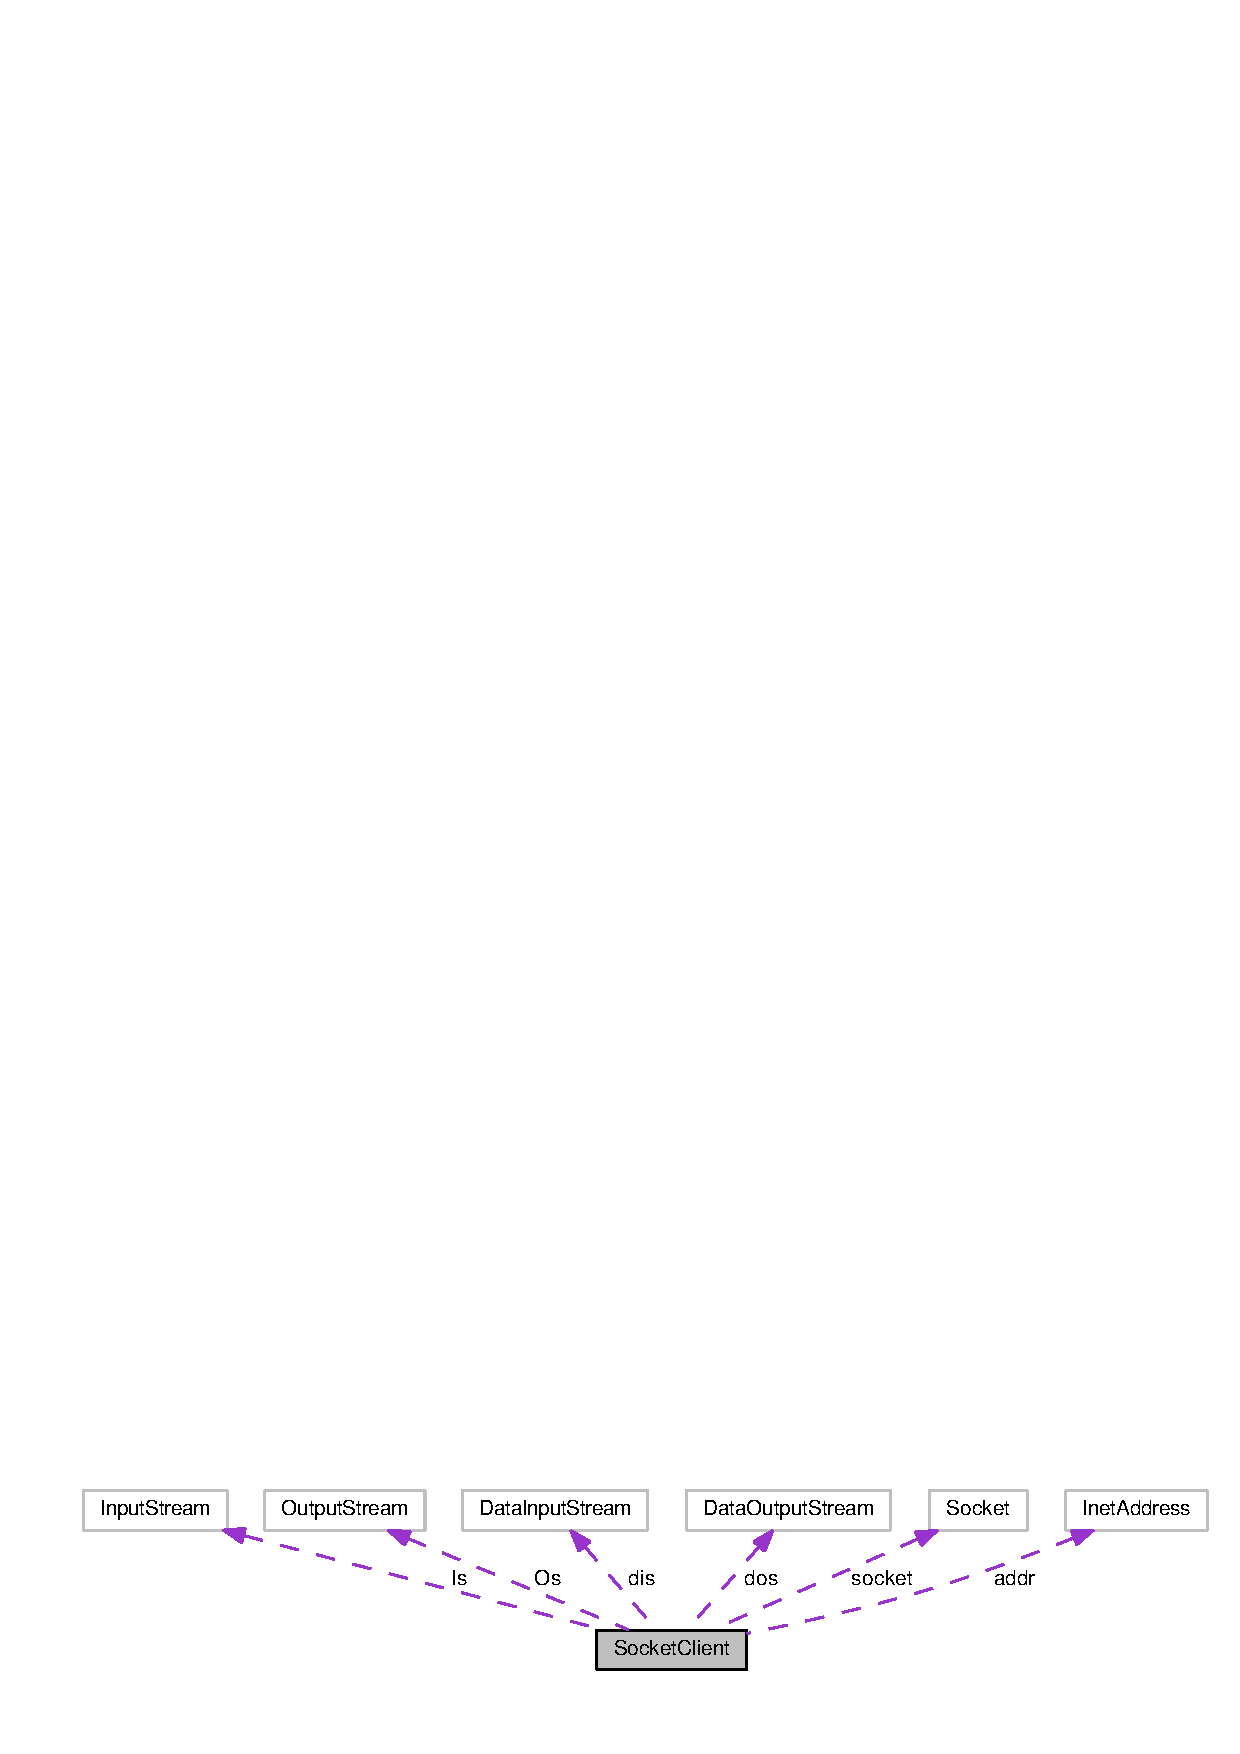
\includegraphics[width=350pt]{class_socket_client__coll__graph}
\end{center}
\end{figure}
\subsection*{公開メンバ関数}
\begin{DoxyCompactItemize}
\item 
void {\bf Receive\-Data} (String arg[$\,$])
\begin{DoxyCompactList}\small\item\em データを受信するメソッド \end{DoxyCompactList}\end{DoxyCompactItemize}
\subsection*{公開変数類}
\begin{DoxyCompactItemize}
\item 
double {\bf velocity}
\begin{DoxyCompactList}\small\item\em 速度 \end{DoxyCompactList}\item 
double {\bf yaw}
\begin{DoxyCompactList}\small\item\em ヨー角 \end{DoxyCompactList}\end{DoxyCompactItemize}


\subsection{詳解}
ソケット通信のクライアント側のクラス 

 Socket\-Client.\-java の 22 行目に定義があります。



\subsection{メソッド詳解}
\index{Socket\-Client@{Socket\-Client}!Receive\-Data@{Receive\-Data}}
\index{Receive\-Data@{Receive\-Data}!SocketClient@{Socket\-Client}}
\subsubsection[{Receive\-Data}]{\setlength{\rightskip}{0pt plus 5cm}void Socket\-Client.\-Receive\-Data (
\begin{DoxyParamCaption}
\item[{String}]{arg[$\,$]}
\end{DoxyParamCaption}
)}\label{class_socket_client_a28def7e2fc6ff0cbeb08c96f39807cfe}


データを受信するメソッド 



 Socket\-Client.\-java の 56 行目に定義があります。



参照先 velocity, yaw.



\subsection{メンバ詳解}
\index{Socket\-Client@{Socket\-Client}!velocity@{velocity}}
\index{velocity@{velocity}!SocketClient@{Socket\-Client}}
\subsubsection[{velocity}]{\setlength{\rightskip}{0pt plus 5cm}double Socket\-Client.\-velocity}\label{class_socket_client_afc3365fa5cdab992bfa54a7b09aa4296}


速度 



 Socket\-Client.\-java の 33 行目に定義があります。



参照元 Receive\-Data().

\index{Socket\-Client@{Socket\-Client}!yaw@{yaw}}
\index{yaw@{yaw}!SocketClient@{Socket\-Client}}
\subsubsection[{yaw}]{\setlength{\rightskip}{0pt plus 5cm}double Socket\-Client.\-yaw}\label{class_socket_client_a5257acafa6dd8303c61bce654272eee1}


ヨー角 



 Socket\-Client.\-java の 34 行目に定義があります。



参照元 Receive\-Data().



このクラス詳解は次のファイルから抽出されました\-:\begin{DoxyCompactItemize}
\item 
{\bf Socket\-Client.\-java}\end{DoxyCompactItemize}

\chapter{ファイル詳解}
\section{E\-V3\-Control\-Client.\-java ファイル}
\label{_e_v3_control_client_8java}\index{E\-V3\-Control\-Client.\-java@{E\-V3\-Control\-Client.\-java}}


E\-V3を制御するクライアント(\-E\-V3)側のメインクラス.  


\subsection*{クラス}
\begin{DoxyCompactItemize}
\item 
class {\bf E\-V3\-Control\-Client}
\begin{DoxyCompactList}\small\item\em クライアント側のメインの処理クラス \end{DoxyCompactList}\end{DoxyCompactItemize}


\subsection{詳解}
E\-V3を制御するクライアント(\-E\-V3)側のメインクラス. \begin{DoxyDate}{日付}
2016.\-01.\-05 
\end{DoxyDate}
\begin{DoxyAuthor}{著者}
H.\-Shigehara 
\end{DoxyAuthor}


 {\bf E\-V3\-Control\-Client.\-java} に定義があります。


\section{Run\-Client.\-java ファイル}
\label{_run_client_8java}\index{Run\-Client.\-java@{Run\-Client.\-java}}


クライアント(\-E\-V3)側の時間をスケジューリングするクラス.  


\subsection*{クラス}
\begin{DoxyCompactItemize}
\item 
class {\bf Run\-Client}
\begin{DoxyCompactList}\small\item\em クライアント側で連続で行う処理を記述したクラス \end{DoxyCompactList}\end{DoxyCompactItemize}


\subsection{詳解}
クライアント(\-E\-V3)側の時間をスケジューリングするクラス. \begin{DoxyDate}{日付}
2016.\-01.\-05 
\end{DoxyDate}
\begin{DoxyAuthor}{著者}
H.\-Shigehara 
\end{DoxyAuthor}


 {\bf Run\-Client.\-java} に定義があります。


\section{Run\-Control\-E\-V3.\-java ファイル}
\label{_run_control_e_v3_8java}\index{Run\-Control\-E\-V3.\-java@{Run\-Control\-E\-V3.\-java}}


E\-V3の走行を制御するクラス  


\subsection*{クラス}
\begin{DoxyCompactItemize}
\item 
class {\bf Run\-Control\-E\-V3}
\begin{DoxyCompactList}\small\item\em E\-V3の走行制御クラス \end{DoxyCompactList}\end{DoxyCompactItemize}


\subsection{詳解}
E\-V3の走行を制御するクラス \begin{DoxyDate}{日付}
2016.\-01.\-05 
\end{DoxyDate}
\begin{DoxyAuthor}{著者}
H.\-Shigehara 
\end{DoxyAuthor}


 {\bf Run\-Control\-E\-V3.\-java} に定義があります。


\section{Socket\-Client.\-java ファイル}
\label{_socket_client_8java}\index{Socket\-Client.\-java@{Socket\-Client.\-java}}


クライアントクラス.\-E\-V3から送信する\-P\-C側のサーバーへ通信する  


\subsection*{クラス}
\begin{DoxyCompactItemize}
\item 
class {\bf Socket\-Client}
\begin{DoxyCompactList}\small\item\em ソケット通信のクライアント側のクラス \end{DoxyCompactList}\end{DoxyCompactItemize}


\subsection{詳解}
クライアントクラス.\-E\-V3から送信する\-P\-C側のサーバーへ通信する \begin{DoxyDate}{日付}
2016.\-01.\-05 
\end{DoxyDate}
\begin{DoxyAuthor}{著者}
H.\-Shigehara 
\end{DoxyAuthor}


 {\bf Socket\-Client.\-java} に定義があります。


%--- End generated contents ---

% Index
\newpage
\phantomsection
\addcontentsline{toc}{chapter}{索引}
\printindex

\end{document}
